为了提高STREAM Triad内核在CPU和GPU上的性能,可以通过将循环转换为paralle\_for内核来计算。\par

STREAM Triad内核可以将其提交到队列,并在CPU上并行执行。STREAM Triad DPC++并行内核的主体看起来就像在CPU上串行C++中执行的STREAM Triad循环的主体,如图16-6所示。\par

\hspace*{\fill} \par %插入空行
图16-6 DPC++ STREAM Triad的paralle\_for内核代码
\begin{lstlisting}[caption={}]
constexpr int num_runs = 10;
constexpr size_t scalar = 3;

double triad(
		const std::vector<double>& vecA,
		const std::vector<double>& vecB,
		std::vector<double>& vecC ) {
			
	assert(vecA.size() == vecB.size() == vecC.size());
	const size_t array_size = vecA.size();
	double min_time_ns = DBL_MAX;
	
	queue Q{ property::queue::enable_profiling{} };
	std::cout << "Running on device: " <<
		Q.get_device().get_info<info::device::name>() << "\n";
	
	buffer<double> bufA(vecA);
	buffer<double> bufB(vecB);
	buffer<double> bufC(vecC);
	
	for (int i = 0; i< num_runs; i++) {
		auto Q_event = Q.submit([&](handler& h) {
			accessor A{ bufA, h };
			accessor B{ bufB, h };
			accessor C{ bufC, h };
			
			h.parallel_for(array_size, [=](id<1> idx) {
				C[idx] = A[idx] + B[idx] * scalar;
			});
		});
	
		double exec_time_ns =
			Q_event.get_profiling_info<info::event_profiling::command_end>() -
			Q_event.get_profiling_info<info::event_profiling::command_start>();
		
		std::cout << "Execution time (iteration " << i << ") [sec]: "
				  << (double)exec_time_ns * 1.0E-9 << "\n";
		min_time_ns = std::min(min_time_ns, exec_time_ns);
	}

	return min_time_ns;
}
\end{lstlisting}

尽管并行内核非常类似于用带有循环的串行STREAM Triad函数,但在CPU上运行速度要快得多,因为paralle\_for允许在多个内核上并行处理数组的不同元素。如图16-7所示,假设有一个系统,其中有一个插槽、四个内核和每个内核有两个超线程,有1024个双精度数据元素要处理。现实中,数据在包含32个数据元素的工作组中处理,这意味着有8个线程和32个工作组。工作组调度可以按循环顺序进行,即thread-id = work-group-id mod 8。每个线程将执行四个工作组,每一轮可以并行执行8个工作组。注意,在本例中工作组是DPC++编译器和运行时会隐式形成的。\par

\hspace*{\fill} \par %插入空行
图16-7 STREAM Triad内核并行的映射
\begin{center}
	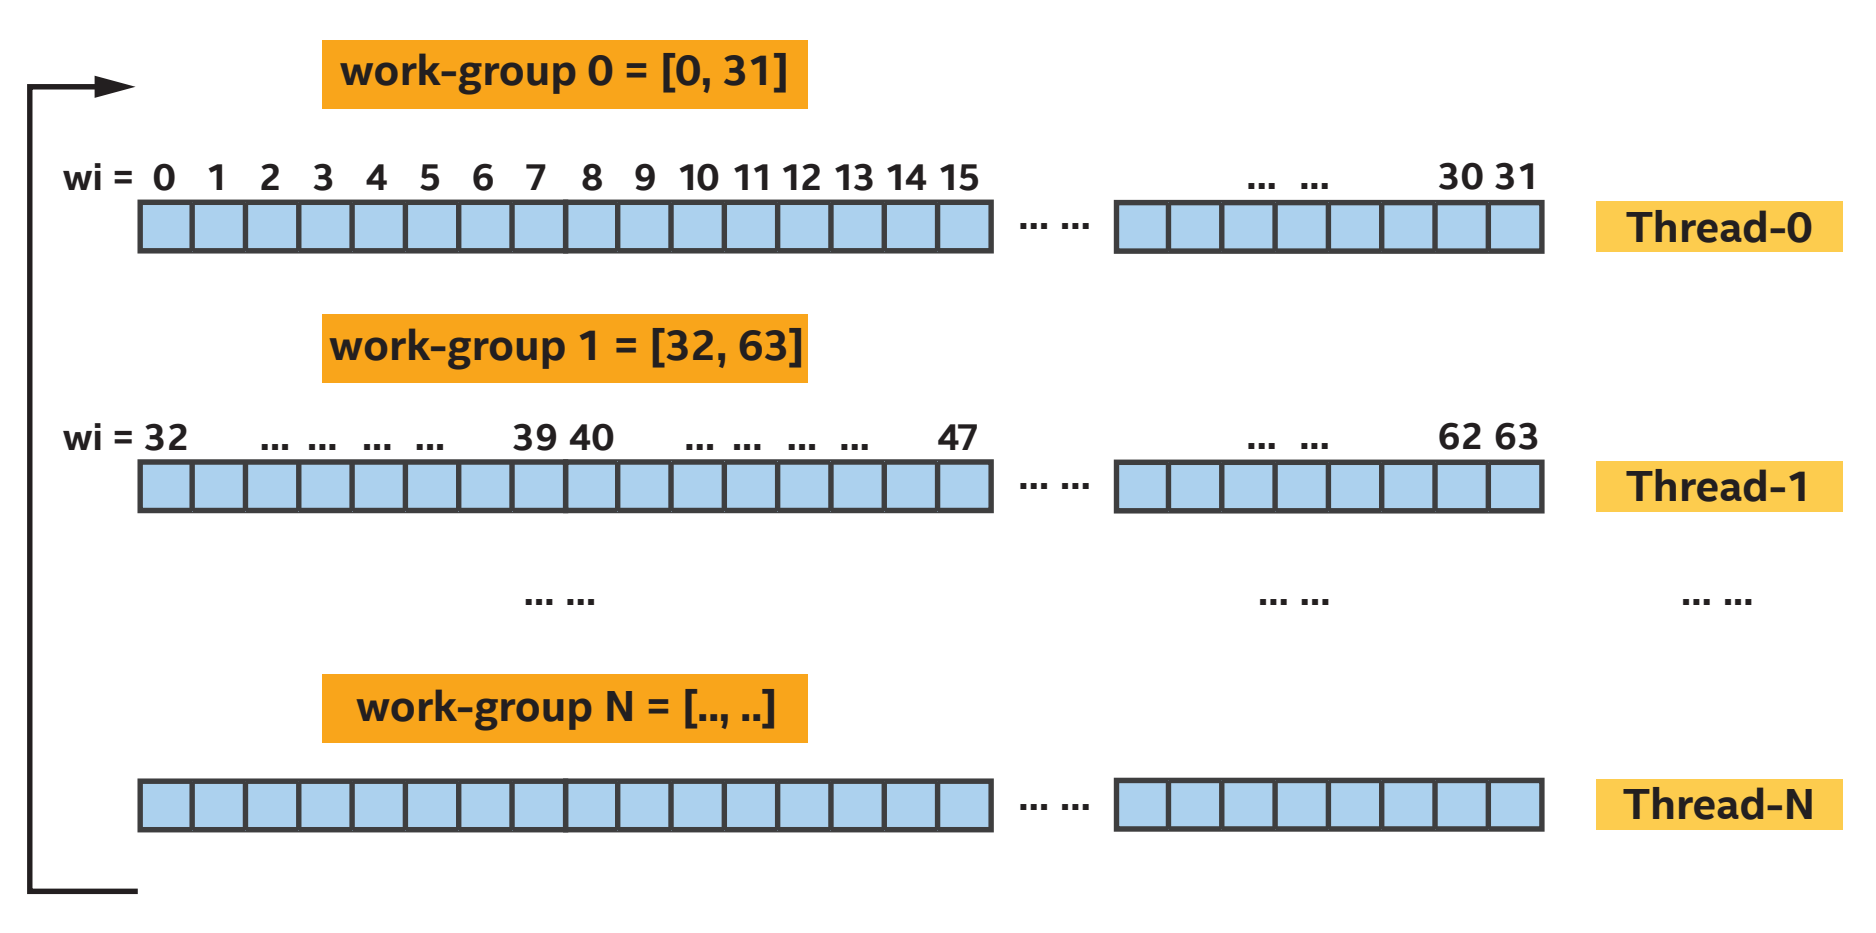
\includegraphics[width=1.0\textwidth]{content/chapter-16/images/5}
\end{center}

注意,在DPC++程序中不需要指定数据元素的分区,以及相应的处理器。这使得DPC++可以灵活地选择,如何在特定的CPU上最好地并行内核。话虽如此,实现可以为程序员提供某种程度的控制,以便性能调优。\par

虽然CPU可能会带来相对较高的线程上下文切换和同步开销,但在处理器上开辟更多的线程是有益的,因为每个处理器核心提供了要执行的工作的选择。如果软件线程正在等待另一个线程产生数据,那么处理器可以切换到另一个准备运行的软件线程,而不会让处理器空闲。\par

\begin{tcolorbox}[colback=blue!5!white,colframe=blue!75!black, title=选择如何绑定和调度线程]
选择一种有效的方案来划分和调度线程之间的工作,对于在CPU和其他设备类型上调优非常重要。接下来的将描述这部分的技术。
\end{tcolorbox}

\hspace*{\fill} \par %插入空行
\textbf{线程的亲和力}

线程亲和力指定特定线程可以在特定的CPU上执行。如果线程在多个核之间移动,性能可能会受到影响,例如:如果线程不在同一个核上执行,如果数据在核之间打乒乓球,则缓存的性能会变得很低。\par

DPC++运行时库支持通过环境变量DPCPP\_CPU\_CU\_AFFINITY、DPCPP\_CPU\_PLACES、DPCPP\_CPU\_NUM\_CUS和DPCPP\_CPU\_SCHEDULE等将线程绑定到内核,但这都不是由SYCL定义。\par

首先是环境变量DPCPP\_CPU\_CU\_AFFINITY。使用这些环境变量进行简单调优,并且对许多应用程序有很大影响。这个环境变量的描述如图16-8所示。\par

\hspace*{\fill} \par %插入空行
图16-8 DPCPP\_CPU\_CU\_AFFINITY环境变量
\begin{table}[H]
	\begin{tabular}{|l|l|}
		\hline
		\textbf{DPCPP\_CPU\_CU\_AFFINITY} & \textbf{描述}                                                                                                                    \\ \hline
		spread                            & \begin{tabular}[c]{@{}l@{}}按照循环顺序将连续线程绑定到从插槽0开始\end{tabular}      \\ \hline
		close                             & \begin{tabular}[c]{@{}l@{}}以循环顺序将连续线程绑定到不同的超线程(以线程0开始)\end{tabular} \\ \hline
	\end{tabular}
\end{table}

\begin{tcolorbox}[colback=green!5!white,colframe=green!75!black]
spread: boundHT = (tid mod numHT) + ( tid mod numSocket) x numHT \\
close: boundHT = tid mod(numSocket x numHT)
\end{tcolorbox}

\begin{itemize}
	\item tid示软件线程标识符。
	\item boundHT表示线程tid绑定到的超线程(逻辑核芯)。
	\item numHT表示每个插槽的超线程数。
	\item numSocket表示系统中的插槽数量
\end{itemize}

假设在一个双核双插槽的超线程系统上,运行一个有8个线程的程序——换句话说,有4个核,总共有8个超线程要进行编程。图16-9展示了线程如何映射到不同DPCPP\_CPU\_CU\_AFFINITY设置的超线程和核芯。\par

\hspace*{\fill} \par %插入空行
图16-9 用超线程将线程映射到内核
\begin{center}
	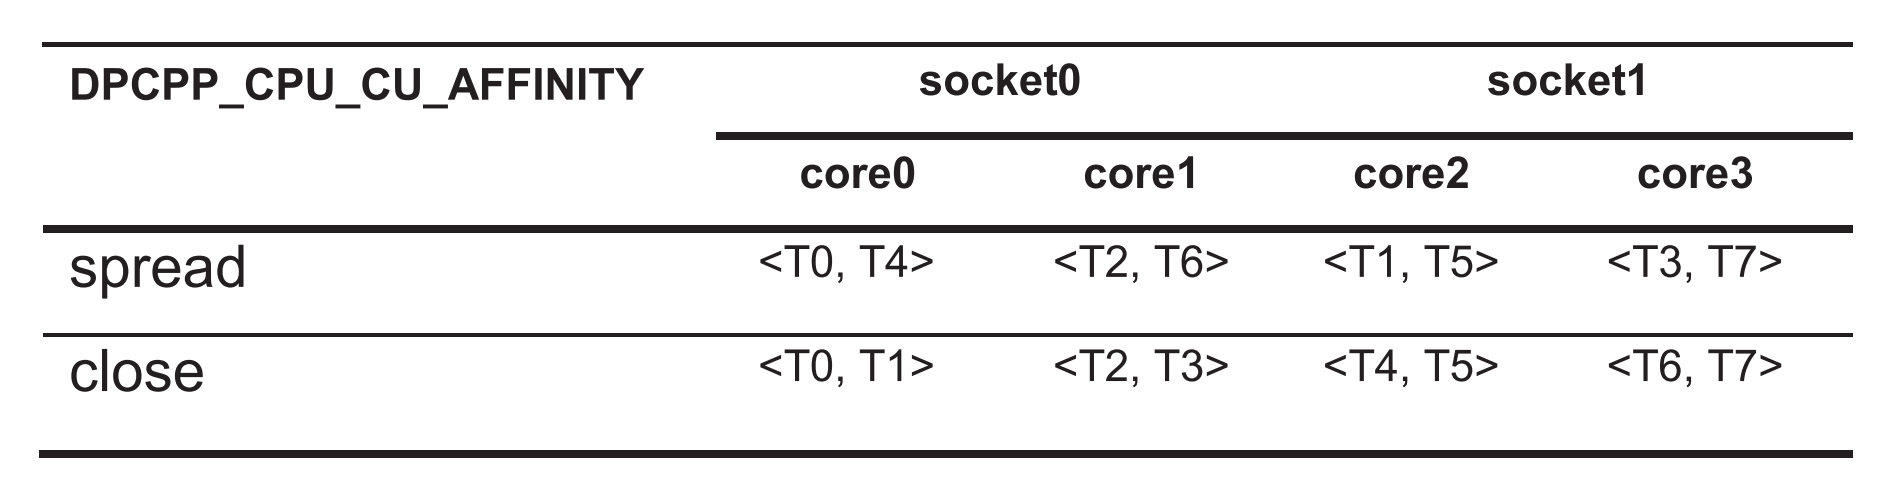
\includegraphics[width=1.0\textwidth]{content/chapter-16/images/6}
\end{center}

除了环境变量DPCPP\_CPU\_CU\_AFFINITY,还有其他支持CPU性能调优的环境变量:\par

\begin{itemize}
	\item DPCPP\_CPU\_NUM\_CUS = [n],它设置用于内核执行的线程数。它的默认值是系统中的硬件线程数。
	\item DPCPP\_CPU\_PLACES = [ sockets | numa\_domains | 	cores | threads ],指定亲和性将被设置的位置,类似于OpenMP 5.1中的OMP\_PLACES。默认设置为“cores”。
	\item DPCPP\_CPUSCHEDULE = [ dynamic | affinity | static ],它指定了调度工作组的算法。默认设置是dynamic。
	\begin{itemize}
		\item dynamic: 启用TBB auto\_partitioner,通常可以平衡工作线程之间的负载。
		\item affinity: 启用TBB affinity\_partitioner,可以改进缓存亲和性,并在将子范围映射到工作线程时使用相应的比例分割。
		\item static: 启用TBB static\_partitioner,尽可能均匀地分布线程之间的负载。
	\end{itemize}
\end{itemize}

TBB使用粒度大小来控制工作拆分,默认粒度大小为1,表示所有工作组都可以独立执行。更多信息可以在spec.oneapi.com/versions/latest/elements/oneTBB/source/algorithms.html\#partitioner找到。\par

缺乏线程关联性调优并不一定性能会低。性能更多地取决于并行执行的线程总数,而不是线程和数据的关联和绑定程度。使用基准测试程序,是确定线程关联是否对性能有影响的一种方法。如图16-1所示,DPC++ STREAM Triad代码在没有线程关联设置的情况下以较低的性能启动。通过控制亲和性设置和通过环境变量(输出如下所示)对软件线程进行静态调度,性能得到了改善:\par

\begin{tcolorbox}[colback=white,colframe=black]
export DPCPP\_CPU\_PLACES=numa\_domains\\
export DPCPP\_CPU\_CU\_AFFINITY=close
\end{tcolorbox}

通过使用numa\_domains对亲和性的位置进行设置,TBB任务领域绑定到numa节点和插槽,并且任务均匀地分布在各个领域。一般情况下,环境变量DPCPP\_CPU\_PLACES建议与DPCPP\_CPU\_CU\_AFFINITY一起使用。这些环境变量设置可以在拥有2个插槽和28个双向超线程内核的Skylake服务器系统上实现了30\%的性能提升,每个插槽中的核芯以2.5GHz运行。但是,我们还可以做得更好,可以进一步提高这个CPU的性能。\par

\hspace*{\fill} \par %插入空行
\textbf{注意与内存的接触}

示例中,初始化循环不是并行的,由主机线程串行执行,所有内存都与主机线程运行的任务相关联。其他任务随后的访问将连接到初始任务(用于初始化)的内存中的数据,这显然不符合性能要求。通过并行化初始化循环来控制跨任务与内存的第一次接触,可以在STREAM Triad内核上实现更高的性能,如图16-10所示。\par

\hspace*{\fill} \par %插入空行
图16-10 STREAM Triad并行初始化内核控制与内存的第一次接触
\begin{lstlisting}[caption={}]
template <typename T>
void init(queue &deviceQueue, T* VA, T* VB, T* VC, size_t array_size) {
	range<1> numOfItems{array_size};
	
	buffer<T, 1> bufferA(VA, numOfItems);
	buffer<T, 1> bufferB(VB, numOfItems);
	buffer<T, 1> bufferC(VC, numOfItems);
	
	auto queue_event = deviceQueue.submit([&](handler& cgh) {
		auto aA = bufA.template get_access<sycl_write>(cgh);
		auto aB = bufB.template get_access<sycl_write>(cgh);
		auto aC = bufC.template get_access<sycl_write>(cgh);
		
		cgh.parallel_for<class Init<T>>(numOfItems, [=](id<1> wi) {
			aA[wi] = 2.0; aB[wi] = 1.0; aC[wi] = 0.0;
		});
	});

	queue_event.wait();
}
\end{lstlisting}

初始化代码中利用并行性可以提高内核在CPU上运行时的性能。在Intel Xeon处理器系统上,这样可以获得了2倍的性能增益。\par

本章最近的几节展示了通过利用线程级并行性,可以有效地利用CPU内核和超线程。然而,还需要利用CPU核心硬件中的SIMD向量级并行性,以实现最佳性能。\par

\begin{tcolorbox}[colback=blue!5!white,colframe=blue!75!black]
DPC++并行内核得益于跨核和超线程的线程级并行!
\end{tcolorbox}





